\section{Method}
\label{sec:method}

\subsection{Setup and Notation}
\label{sec:method:setup}

% 十修: B8 — backbone citation + availability (verified against the local
% checkpoint: Flux2KleinPipeline, flux-2-klein-9b.safetensors).
We target training-free style transfer on Klein~9B
(FLUX.2~[klein]~9B~\cite{flux2klein2025}, an open-weights
MM-DiT rectified-flow model~\cite{esser2024scaling} with 8 double-stream blocks
and 24 single-stream blocks).
Given a text prompt~$p$ and a style reference image~$x_s$, the goal is to
generate an image that matches the semantic content of~$p$ while adopting
the visual style of~$x_s$, without modifying any model weights.

\paragraph{Notation}
Let $z_t \in \mathbb{R}^{L \times D}$ denote the packed image latent at
denoising timestep~$t$, $L$ tokens of dimension~$D$.
$z_s = \text{VAE}(x_s)$ is the style-image encoding.
Self-attention at layer~$\ell$ produces
$Q^{(\ell)}, K^{(\ell)}, V^{(\ell)} \in \mathbb{R}^{H \times L \times d}$
($H$ heads, $d = D/H$); subscripts~$c$ and~$s$ denote content and style
branches.
We run 25 denoising steps with guidance scale 3.5 at $512 \times 512$
on a single H200 GPU, fixed seed~43.

% ─────────────────────────────────────────────────────────────────────────────
\subsection{Attention Interpolation Baseline}
\label{sec:method:baseline}

The canonical training-free approach blends content and style attention
features via a scalar interpolation:
\begin{align}
  \hat{z}_t &= (1-\beta)\,\text{Attn}(Q_c, K_c, V_c) \notag\\
            &\quad + \beta\,\text{Attn}(Q_c, K_s, V_s),
  \qquad \beta \in [0,1].
  \label{eq:injection}
\end{align}
This requires no optimization (one additional style forward pass per step)
and represents the broad class of injection-based training-free
methods~\cite{hertz2024style,vshuffle2025,dualrf2025}.

\emph{Limitation.}
The latent update is a single feedforward operation.
There is no iterative feedback to reinforce the style signal or propagate it
across the spatial token grid.
On our benchmark, best-effort injection achieves CSD~$< 0.15$, giving only faint
hue shifts with no texture structure.
We trace this failure directly to the absence of backpropagation, as detailed
in the next section.

% ─────────────────────────────────────────────────────────────────────────────
\subsection{Spatial Coherence of Latent Updates}
\label{sec:method:gap}

\begin{figure*}[t]
  \centering
  \begin{subfigure}{0.48\textwidth}
    \centering
    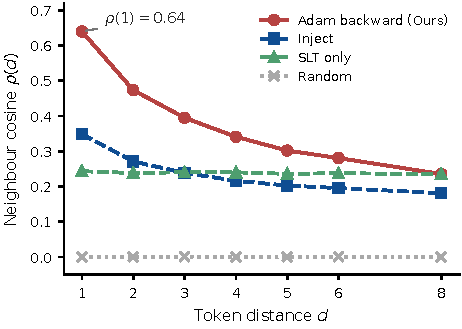
\includegraphics[width=\linewidth]{fig/figure/fig8a_spatial_decay.pdf}
    \caption{Measured spatial neighbour cosine $\rho(d)$ vs.\ token distance.
    Adam-backward updates are strongly coherent for neighbours ($\rho{=}0.64$)
    and stay coherent over distance; injection ($0.35$) is weaker, per-token SLT
    is flat-low ($0.24$, no local structure), and a random control is zero.}
    \label{fig:spatial_decay}
  \end{subfigure}\hfill
  \begin{subfigure}{0.48\textwidth}
    \centering
    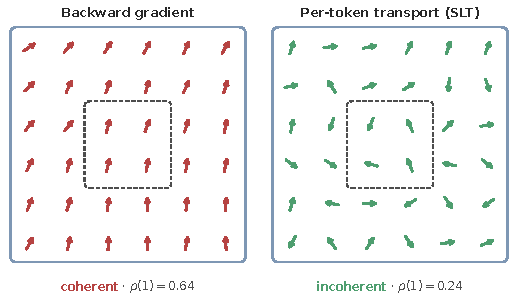
\includegraphics[width=\linewidth]{fig/figure/concept_spatial.pdf}
    \caption{Mechanism: the value-path self-attention Jacobian couples
    neighbouring tokens---adjacent content keys are nearly identical, so
    backpropagation delivers near-identical gradient directions to spatially
    adjacent positions, whereas per-token transport (SLT) has no such
    coupling ($\rho{=}0.24$; Table~\ref{tab:spatial_proof}).}
    \label{fig:concept_spatial}
  \end{subfigure}
  \caption{Spatial coherence of latent updates: \textbf{(a)} the
  \emph{measured} coherence $\rho(d)$ and \textbf{(b)} the value-path Jacobian
  \emph{mechanism} that produces it. Detailed per-token coherence maps
  are in the supplement (Fig.~\ref{fig:pca_maps}).}
  \label{fig:spatial_coherence}
\end{figure*}

% 十修: premise sentence rewritten for consistency with our own unified-protocol
% measurements (tab:percat, Sec.~\ref{sec:exp}), where the strongest trained
% baseline (CSGO) reaches only a mean CSD of 0.506; the 0.6--0.8 figure is what
% trained methods self-report under their own (non-unified) protocols.
Trained style methods produce coherent brushstroke texture, with
self-reported style fidelity of CSD~$\approx 0.6$--$0.8$ under their own
protocols; under our unified protocol the strongest baseline reaches only a
mean of $0.506$ (Table~\ref{tab:percat}).
To understand why, consider the gradient that flows back through the
self-attention module during fine-tuning.
Backpropagation couples tokens through the \emph{value path} of attention:
token $i$'s value contributes to the output at every position $j$ with
weight $A_{ji}$, so the gradient arriving at token $i$ aggregates residuals
from \emph{all} positions, weighted by the $i$-th column of the attention
matrix.
Neighboring tokens $(i,\,i{+}1)$ carry nearly identical keys—RoPE encodes
adjacent grid positions with nearly identical rotation
matrices~\cite{su2024rope} ($\|\mathbf{R}(\mathbf{p}_i){-}\mathbf{R}(\mathbf{p}_{i+1})\|_F
\approx 0.098$) and denoising latents are spatially smooth—so adjacent
attention columns nearly coincide and adjacent tokens receive nearly
identical gradient signals.
These correlated updates cause neighboring tokens to be nudged in the
\emph{same direction}, producing the long-range spatial correlations that
define painterly texture.

\paragraph{Empirical confirmation}
We measure this directly via the \emph{spatial neighbor cosine}:
\begin{equation}
  \rho = \frac{1}{|\mathcal{N}|} \sum_{(u,v) \in \mathcal{N}}
         \cos(\delta_{u},\, \delta_{v}),
  \label{eq:rho}
\end{equation}
where $\delta_{u}$ is the per-token latent update at grid position $u$ and
$\mathcal{N}$ is the set of horizontally and vertically adjacent position
pairs on the $32 \times 32$ token grid
($|\mathcal{N}| = 2 \times 31 \times 32$).
Results are shown in Table~\ref{tab:spatial_proof} and
Fig.~\ref{fig:spatial_coherence}a, with the convergence and gradient-source
analyses in Fig.~\ref{fig:spatial_proof}; the detailed per-token
update-direction coherence maps appear in the supplement
(Fig.~\ref{fig:pca_maps}).
Fig.~\ref{fig:spatial_proof}a shows that Backward$+$SLT (ours) converges
fastest, reaching at $N{=}2$ the style loss that backward-only optimization
requires $N{\approx}4$ to match, while the gradient-free Inject and SLT-only
baselines cannot iterate.
Fig.~\ref{fig:spatial_proof}b isolates the source of the coherence: shuffling
the spatial order of the style $K/V$ leaves $\rho$ unchanged ($0.654$ vs.\
$0.654$), ruling out the style-image layout; removing style $K/V$ entirely
collapses coherence to $\rho{=}0.168$, whereas a single-patch style loss
recovers most of it ($\rho{=}0.628$)---confirming that the self-attention
backward pass propagates the style signal globally through the value path.

\begin{figure}[tb]
  \centering
  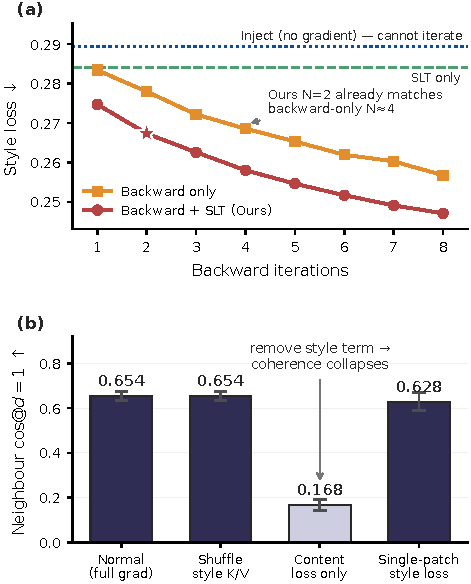
\includegraphics[width=\linewidth]{fig/figure/fig3_spatial_proof.pdf}
  \caption{Style-loss convergence (a) and the gradient-source analysis
  of spatial coherence (b); see Sec.~\ref{sec:method:gap}.}
  \label{fig:spatial_proof}
\end{figure}

\begin{table}[h]
  \centering
  \caption{Spatial neighbor cosine $\rho$ ($d{=}1$) by gradient source,
           measured at the first Adam iteration and averaged over 6
           content--style pairs (4 pairs for the content-loss-only and
           stop-grad-$Q$ conditions).
           Fig.~\ref{fig:spatial_proof}b visualizes the gradient-source
           conditions on the 4-pair ablation set (first iteration); minor
           value differences from this table reflect the smaller sample.
           Higher = more spatially coherent = brushstroke texture.}
  \label{tab:spatial_proof}
  \footnotesize
  \begin{tabular}{lcc}
    \toprule
    Gradient condition & $\rho$ & Interpretation \\
    \midrule
    Random direction (control)   & $0.00$  & No structure \\
    SLT per-token OT             & $0.24$  & Accidental proximity \\
    Content-loss-only gradient   & $0.17$  & Weak self-coupling \\
    Adam full gradient (backprop)& $0.64$  & \textbf{Value-path Jacobian} \\
    Stop-grad-$Q$ gradient       & $0.65$  & Value-path dominant \\
    \bottomrule
  \end{tabular}
\end{table}

The $2.6\times$ gap between Adam gradients ($\rho = 0.64$) and OT updates
($\rho = 0.24$) is the quantitative signature of the backpropagation gap:
training-free OT operates token by token independently, whereas backward-pass
gradients couple neighbors through the shared attention pattern and are
therefore $2.6\times$ more spatially coherent.

\begin{proposition}[Spatial gradient coherence]
\label{prop:spatial}
Let $g_i = \partial\mathcal{L}_\mathrm{style}/\partial z_i$ be the gradient of
the style-alignment loss at token $i$.
The content self-attention produces a \emph{value-path coupling term}
\begin{equation}
  g_i^{\mathrm{val}}
  = -2W_V \sum_{j} A_{ji}^c\, R_j,
  \label{eq:gval}
\end{equation}
where $A^c$ is the content attention matrix and $R = O_s - O_c$.
If content keys satisfy the $\epsilon$-spatial smoothness condition
$\|K_{c,i} - K_{c,i+1}\|_2 \leq \epsilon\sqrt{d}$ (with
$q_{\max}\epsilon \leq 1$, $q_{\max}$ the maximal query norm), then
\begin{equation}
  \cos\!\bigl(g_i^{\mathrm{val}},\, g_{i+1}^{\mathrm{val}}\bigr)
  \;\geq\; 1 - \tfrac{C\,\epsilon^2\|R\|_F^2}{\|g^{\mathrm{val}}\|_{\min}^2},
  \qquad C = 2e^2\|W_V\|_2^2\,q_{\max}^2\,L.
  \label{eq:prop1}
\end{equation}
SLT updates have $\partial\Delta_i/\partial z_j = 0$ for $i \neq j$ (with the
transport plan $T$ held fixed during the update, as in our implementation),
so no analogous coupling exists; their spatial coherence depends only on
accidental proximity of transport targets.
\end{proposition}

The key step (Appendix~\ref{app:jacobian}) is that $g_i^{\mathrm{val}}$
is a weighted average of the residual $R$ over \emph{all} positions, with
column weights $A_{ji}^c$ that are nearly equal for adjacent $i$ whenever
content keys are spatially smooth.
This smoothness is structurally motivated in MM-DiT~\cite{esser2024scaling}:
the RoPE rotation-difference bound~\cite{su2024rope}
$\|R(\mathbf{p}_i){-}R(\mathbf{p}_{i+1})\|_F \approx 0.098$ constrains the
positional part of the key difference $\|K_{c,i}{-}K_{c,i+1}\|$, and the
spatial smoothness of denoising latents constrains the remainder; the
resulting attention-weight difference is bounded by the softmax
logit-difference argument in Appendix~\ref{app:jacobian}.
SLT operates entirely in token-distribution space and bypasses the attention
Jacobian; $\partial\Delta_i/\partial z_j = 0$ for $i \neq j$ by construction,
which accounts for the $2.6\times$ gap in $\rho$.

\paragraph{Ablation --- which gradient path drives spatial coherence}
To isolate the value-path contribution experimentally, we compare three gradient
conditions: (i) \emph{Normal} (full gradient), (ii) \emph{Stop-grad-$Q$}
(Q detached before the attention product, removing the query-side gradient
path), and
(iii) \emph{Random direction} (control).
Normal and Stop-grad-$Q$ achieve identical spatial coherence
($\rho \approx 0.65$) at every iteration, while Random yields $\rho \approx 0.00$
(see Supplementary Fig.~\ref{fig:jacobian_ablation}).
The query-side Jacobian path is therefore \emph{not} the source of spatial
coherence; combined with the empirical subdominance of the key-side term
($\|g^K\|/\|g^{\mathrm{val}}\| < 0.15$, Appendix~\ref{app:jacobian}), this
identifies the value-path term $g_i^{\mathrm{val}}$ (Eq.~\ref{eq:gval}) as
the responsible mechanism, consistent with Proposition~\ref{prop:spatial}.

% ─────────────────────────────────────────────────────────────────────────────
\subsection{Adam-in-Loop Latent Optimization}
\label{sec:method:adam}

\begin{figure}[t]
  \centering
  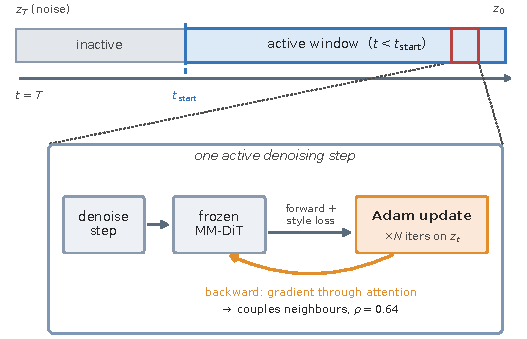
\includegraphics[width=\linewidth]{fig/figure/concept_adam.pdf}
  \caption{The Adam-in-loop schedule: $N$ Adam iterations inside each
  active denoising step ($t<t_\text{start}$).}
  \label{fig:concept_adam}
\end{figure}

The diagnosis suggests a direct fix: run backpropagation through the frozen
model at each denoising step, optimizing only the latent $z_t$.
No weights change; the gradient serves purely to propagate spatial coherence
into the latent update.
We call this \textbf{Adam-in-loop}. Fig.~\ref{fig:concept_adam} illustrates the schedule: at every active
step, gradients backpropagated through the frozen MM-DiT update the content
latent, supplying the cross-token spatial coupling.

\paragraph{Formulation}
At each denoising timestep $t < t_\text{start}$, after the standard denoising
update, we run $N$ Adam steps on a style-alignment loss:
\begin{multline}
  \mathcal{L}_\text{style} = \sum_{\ell}
  \bigl\|\text{Attn}(Q_c^{(\ell)}, K_s^{(\ell)}, V_s^{(\ell)}) \\
         - \text{Attn}(Q_c^{(\ell)}, K_c^{(\ell)}, V_c^{(\ell)})\bigr\|_1,
  \label{eq:adam_loss}
\end{multline}
with an $\ell_1$ content-anchor term to resist structural drift
($\mathcal{L} = w_s\mathcal{L}_\text{style} + w_c\mathcal{L}_\text{cnt}$,
$w_s{=}2.0$, $w_c{=}1.5$, lr$\,{=}\,0.03$).
Gradients flow through the content forward pass and through the
self-attention Jacobian, providing the spatial coherence that injection cannot.

% 十一修 评阅#6: 本小节原 \paragraph{Results}（迭代数-质量对照 + tab:iter_tradeoff
% 表 + Adam-8 保守配置选择规则）整体移入 Sec.4.5 Efficiency Analysis；第 3 节只留
% 原理与指针。
Iteration-count and equal-budget comparisons against Adam-only---and the
selection rule for the conservative Adam-8 reference configuration used in
Tables~\ref{tab:main} and~\ref{tab:ablation}---are analyzed in
Sec.~\ref{sec:exp:efficiency} (Table~\ref{tab:iter_tradeoff},
Fig.~\ref{fig:iter_tradeoff}).

% ─────────────────────────────────────────────────────────────────────────────
\subsection{Frequency-Domain Sinkhorn Loss}
\label{sec:method:freq}

\begin{figure}[t]
  \centering
  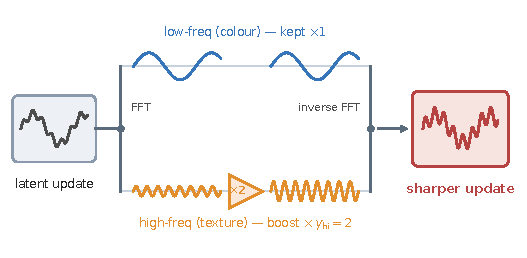
\includegraphics[width=\linewidth]{fig/figure/concept_freq.pdf}
  \caption{The frequency-domain Sinkhorn loss: the high-frequency band
  is amplified ($\gamma_\text{hi}{=}2$) before transport.}
  \label{fig:concept_freq}
\end{figure}

Before turning to Adam's efficiency bottleneck (Sec.~\ref{sec:method:slt}), we
describe one refinement internal to the style loss itself. Fig.~\ref{fig:concept_freq} sketches the mechanism: amplifying the
high-frequency (texture) band before transport sharpens brushstroke detail
without disturbing the global color alignment.
Within Adam's style loss $\mathcal{L}_\text{style}$, we decompose the latent
into low- and high-frequency components via per-channel frequency separation
and apply boosted transport weighting to the high-frequency component:
\begin{equation}
  \mathcal{L}_\text{style} = \mathcal{L}_\text{lo} + \gamma_\text{hi}\,\mathcal{L}_\text{hi},
  \quad \gamma_\text{hi} = 2.0.
  \label{eq:freq}
\end{equation}
The low-frequency component captures global tone; the high-frequency component
carries fine-grained texture: thin brushstrokes, sharp grain, edge details.
Standard $\ell_1$ loss, averaged over all frequency bands, under-weights
high-frequency terms because they carry less energy; the boost coefficient
$\gamma_\text{hi}=2.0$ corrects this, recovering fine-grained detail that
would otherwise be smoothed by the gradient averaging in Adam.
Ablation (Sec.~\ref{sec:ablation}) shows $+0.4\%$ CSD versus no boost.

% ─────────────────────────────────────────────────────────────────────────────
\subsection{Sinkhorn Latent Transport}
\label{sec:method:slt}

\begin{figure}[t]
  \centering
  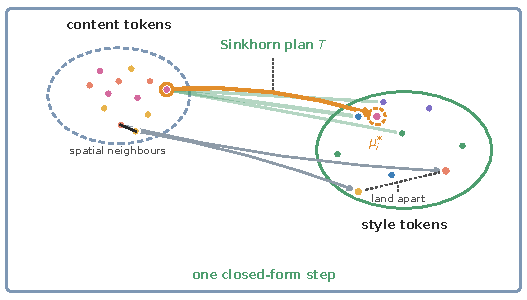
\includegraphics[width=\linewidth]{fig/figure/concept_slt.pdf}
  % 十一修(2026-07-06 评阅#3 二改): 图内三行说明文字删除，信息移入本 caption；
  % 图只保留六个短标签 + "one closed-form step" 一句 takeaway。
  \caption{Sinkhorn Latent Transport in the latent colour plane: the
  doubly-stochastic plan $T$ (green fan, line width $\propto T_{ij}$) matches
  each content token to the whole style distribution and moves it to its
  OT-weighted target $\mu^{*}_{i}$ in one closed-form AdaIN step
  ($\approx$0.1\,ms, no forward pass, no attention Jacobian). Adjacent tokens
  (solid link) are transported independently and land apart: colour is aligned
  but no cross-token coupling arises ($\rho(1){=}0.24$), hence no texture.}
  \label{fig:concept_slt}
\end{figure}

\paragraph{Gradient budget of early Adam iterations}
Profiling the Adam-in-loop gradient at each iteration reveals that the first
2--3 steps are dominated by the correction of low-frequency color mismatch
between $z_t$ and $z_s$.
Color distribution alignment is a global, per-channel operation that is
inefficient to perform via spatially local per-token gradient steps.
If this phase could be replaced by a single closed-form operation,
subsequent Adam iterations could begin immediately in the texture regime.

\paragraph{SLT formulation}
Optimal transport provides exactly this: the doubly-stochastic transport plan
$T = \text{Sinkhorn}(\tilde{S}/\tau)$ computed from the cosine-similarity matrix
$\tilde{S}_{ij} = \cos(\tilde{z}_t[i],\, \tilde{z}_s[j])$
over high-frequency residuals $\tilde{z} = z - \bar{z}$ (spatial mean subtracted)
globally matches each content token to a distribution over style tokens in a single
operation.
We use $T$ to derive per-token style distribution targets and apply
adaptive instance normalization~\cite{huang2017arbitrary}:
\begin{equation}
  \hat{z}_t[i] = \sigma^*_i\,\frac{z_t[i] - \mu_t}{\sigma_t} + \mu^*_i,
  \quad
  z_t \leftarrow (1-\alpha)\,z_t + \alpha\,\hat{z}_t,
  \label{eq:slt}
\end{equation}
where $\mu^*_i = \sum_j T_{ij}\,z_s[j]$ and $\sigma^*_i = \sqrt{\sum_j T_{ij}\,z_s[j]^2 - (\mu^*_i)^2}$
are the OT-weighted per-token target mean and standard deviation,
and $\mu_t, \sigma_t$ are the global statistics of the content latent
($\alpha{=}0.10$, $\tau{=}0.02$, $n_{\mathrm{iters}}{=}10$).
Compared to directly interpolating token embeddings
($z_t \leftarrow (1-\alpha)z_t + \alpha\,Tz_s$),
this OT-AdaIN formulation transfers per-token distribution statistics rather
than embedding values, preserving content structure while ensuring
global color alignment.
The doubly-stochastic constraint
($\sum_j T_{ij}{=}1$, $\sum_i T_{ij}{=}1$)
ensures every style token contributes to the transported statistics,
preventing the mode collapse that row-only softmax normalization permits.
The Sinkhorn solve runs in $\approx 0.1$~ms with no model forward pass;
the style features $z_s$ are already available from the attention injection
branch, so SLT adds zero additional forward passes. Fig.~\ref{fig:concept_slt} depicts the transport: it operates
directly in token space, bypassing the attention Jacobian---resolving color
cheaply while, by construction, producing no cross-token spatial coupling.

% 十一修 评阅#6: 原 \paragraph{SLT result and its limitation} 的实验数字
% （CSD 0.298 / ≈2.2s）移出——CSD 0.298 已由 Sec.5 的 "No Adam (SLT only)"
% 消融报告、wall-clock 已由 Sec.4.5 报告；本处只保留机制层面的局限性论述。
\paragraph{Structural limitation}
By construction the OT assignment is per-token independent: nothing
couples the update of token~$i$ to its neighbor's state, so SLT updates carry
low spatial coherence ($\rho = 0.24$, $2.6\times$ below Adam gradients;
Table~\ref{tab:spatial_proof}) and no spatially coherent structures emerge.
SLT resolves the global distribution gap but cannot generate \emph{local
structural correlations}; its measured quality ceiling and wall-clock cost are
quantified in the ablation (Sec.~\ref{sec:ablation}) and the efficiency
analysis (Sec.~\ref{sec:exp:efficiency}).

% ─────────────────────────────────────────────────────────────────────────────
\subsection{Layout Residual Suppression}
\label{sec:method:lrs}

Style K/V tensors carry both texture statistics and the spatial layout of the
reference image.
Injecting them unmodified causes content objects to drift toward reference
subject positions (\emph{layout leakage}).

\paragraph{Decomposition}
Any style key tensor decomposes as
$K_s^{(\ell)} = \mu_K^{(\ell)} + R_K^{(\ell)}$,
where $\mu_K^{(\ell)}$ is the token mean (permutation-invariant, carries
global style statistics) and $R_K^{(\ell)} = K_s - \mu_K$ is the
position-specific residual (carries spatial layout).

\paragraph{LRS suppression}
We attenuate the layout residual with a depth-dependent coefficient:
\begin{equation}
  K_s^{(\ell)\prime} = \mu_K^{(\ell)} + \gamma^{(\ell)}\,
                       (K_s^{(\ell)} - \mu_K^{(\ell)}),
  \label{eq:lrs}
\end{equation}
with the same transform applied to $V_s$; $\gamma^{(\ell)}$ is linearly
interpolated over block depth from $\gamma_\text{shallow}=0.7$ to
$\gamma_\text{deep}=0.5$.
Deeper blocks, whose features are more layout-specific, are attenuated more
strongly; the retained residual preserves texture directionality cues while
suppressing the layout leakage that causes subject-position drift.

\paragraph{Why this suppresses leakage}
Layout leakage arises because a content query $q_i$ attends to the style keys
with \emph{position-dependent} weights, importing \emph{where} the reference's
structures sit. Decompose the pre-softmax logit under \cref{eq:lrs}:
\begin{equation}
  q_i^\top K_{s,j}^{(\ell)\prime}
    \;=\; \underbrace{q_i^\top \mu_K^{(\ell)}}_{\text{constant in } j}
        \;+\; \gamma^{(\ell)}\, q_i^\top R_{K,j}^{(\ell)} .
  \label{eq:lrs_logit}
\end{equation}
The first term is identical for every style token $j$: it shifts all logits
equally and therefore \emph{cancels} in the softmax. Only the second,
position-varying term selects which style positions a token attends to, and its
dispersion across positions is scaled by $\gamma^2$:
\begin{equation}
  \operatorname{Var}_j\!\big(q_i^\top K_{s,j}^{(\ell)\prime}\big)
    \;=\; \big(\gamma^{(\ell)}\big)^2\,
          \operatorname{Var}_j\!\big(q_i^\top R_{K,j}^{(\ell)}\big).
  \label{eq:lrs_var}
\end{equation}
As $\gamma^{(\ell)}\!\to\!0$ the attention distribution over style tokens
becomes uniform: the output still draws on the global style statistics carried by
$\mu_K^{(\ell)}$ (palette, texture energy) but no longer on the \emph{spatial
arrangement} encoded in $R_K^{(\ell)}$, so the layout residual cannot propagate
into the generated image. As $\gamma^{(\ell)}\!\to\!1$ the full layout returns.
LRS therefore continuously trades layout leakage against texture retention, and
the depth schedule attenuates most strongly in the deep, layout-specific blocks
while preserving the shallow-block residual that carries brushstroke
directionality. Appendix~\ref{app:lrs_proof} makes the leakage bound precise.

% ─────────────────────────────────────────────────────────────────────────────
% ARCHITECTURE FIGURE
% ── IMAGE GENERATION PROMPT (vector diagram, export as PDF or high-res PNG) ─
%
%   Two-panel figure (top + bottom), see reference HTML: fig/architecture.html
%
%   TOP PANEL — Overall pipeline (horizontal flow):
%     Left: style branch
%       [x_s image icon] →[VAE (blue)]→ z_s →[Frozen Φ, dashed gray box]→ K_s,V_s →[LRS (green box)]→ K_s',V_s'
%     Center: denoising timeline
%       [p + z_T~N(0,I)] →───────────── ×25 denoising steps ─────────────→ z_0 →[VAE⁻¹]→ [output image]
%       Highlight active region (t < 850) with purple dashed rectangle; connect to bottom panel with bracket lines.
%     Style branch K_s',V_s' feeds down into the active region.
%
%   BOTTOM PANEL — Per-step module (horizontal flow, same color scheme):
%     z_t →[LRS block, green]→[SLT block, orange]→[Adam×2 block, red]→[Result box, purple] z_t'
%     LRS: "K_s' = μ_K + γ^(ℓ)·R_K  (γ^(ℓ): 0.7→0.5 by depth)"
%     SLT: "T=Sinkhorn(cos(z̃_t,z̃_s)/τ) · OT-AdaIN(z_t;T) · α=0.10 τ=0.02"
%          ρ badge: "ρ_SLT=0.24 (closes color gap, no J_attn)"
%     Adam×2: "∇_z L through J_attn · L=2.0L_sty+1.5L_cnt · freq-Sinkhorn boost γ_hi=2.0"
%             ρ badge: "ρ_Adam=0.64 → brushstrokes"
%             backprop curve arrow labeled "∂L/∂z_t"
%     Result: mini table (Inject <0.15 / SLT 0.298 / Adam-8 0.608 / Ours 0.640)
%             "+5.2% CSD vs Adam-8 · 2.5× lower fwd cost; +16.6% CSD at equal budget"
%
%   COLOR SCHEME: blue=style/frozen, green=LRS, orange=SLT, red=Adam, purple=contribution border
%   FONT: Helvetica/Arial 10–12pt, no serifs
%   EXPORT: fig/architecture.pdf at 300 dpi width ≥ 17cm (TPAMI double-column)
%   TOOL: Inkscape / draw.io / matplotlib + patches / TikZ
%   PREVIEW: fig/architecture.html (open in browser)
% ─────────────────────────────────────────────────────────────────────────────
% (framework overview figure moved to the Introduction as Fig.~\ref{fig:architecture})

% ─────────────────────────────────────────────────────────────────────────────
\subsection{Hyperion Pipeline: SLT Pre-Alignment with Adam Refinement}
\label{sec:method:hybrid}

\begin{figure*}[!t]
  \centering
  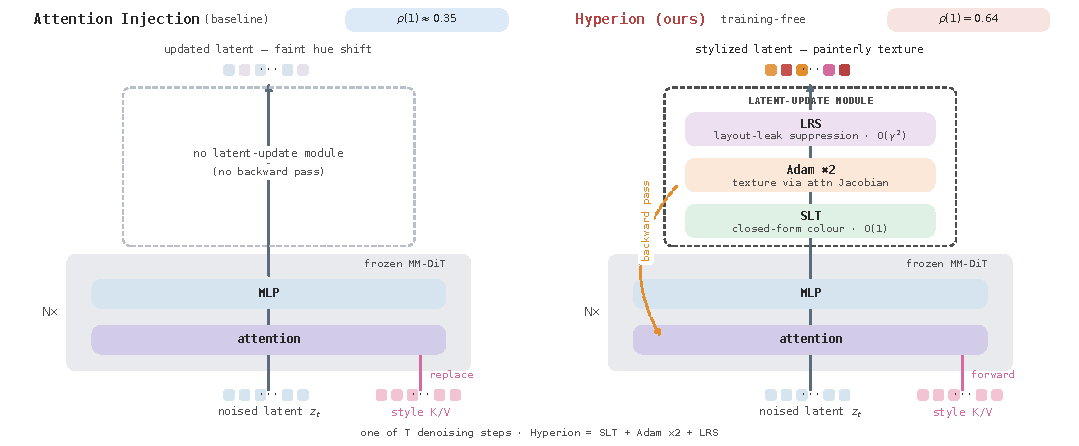
\includegraphics[width=\textwidth]{fig/figure/fig_framework_v4_pastel.pdf}
  \caption{One denoising step of the attention-injection baseline
  (left) and Hyperion (right); the two routes differ only in the
  latent-update module above the frozen backbone.}
  \label{fig:step_compare}
\end{figure*}

\paragraph{Design}
The two mechanisms are complementary with non-overlapping failure modes:
SLT is efficient at what Adam is slow at (global color alignment),
while Adam produces what SLT cannot (spatial texture coherence via the Jacobian).
The Hyperion pipeline (Fig.~\ref{fig:architecture}) chains them within each
denoising step in three stages.
Fig.~\ref{fig:step_compare} draws one such step next to the injection
baseline: the two routes differ only in whether the latent-update module fills
the lane above the frozen backbone.
Both panels share the same skeleton---the noised latent $z_t$ and the
style $K/V$ tokens enter the frozen MM-DiT---but injection applies no latent
update and yields only a faint hue shift ($\rho(1){\approx}0.35$), whereas the
chain SLT${\to}$Adam${\times}2{\to}$LRS produces spatially coherent texture
($\rho(1){=}0.64$).
First, the style branch supplies $K_s^{(\ell)}, V_s^{(\ell)}$ and LRS
layout-leakage suppression is applied (Sec.~\ref{sec:method:lrs}).
Second, the SLT pre-alignment (Eq.~\ref{eq:slt}, $\alpha=0.10$)
collapses the color distribution gap before Adam begins.
Third, two Adam steps are run on
$\mathcal{L} = 2.0\,\mathcal{L}_\text{style} + 1.5\,\mathcal{L}_\text{cnt}$
with frequency-domain Sinkhorn loss (Sec.~\ref{sec:method:freq}); because
the color gap is already closed, both iterations are spent entirely on texture,
generating brushstrokes through the Jacobian.
% 十修: disclose the two auxiliary AdaIN color operations (previously present
% in code but not in the algorithm/text); ablation numbers from the n=40
% color-mechanism decomposition (t2i_sltadam.csv: ota_a01 vs.\ ota_noAdain).
For completeness, we also disclose two auxiliary color operations that
bookend this loop, both applied unconditionally for Hyperion: a per-step
AdaIN warm-start toward the (noised) style latent statistics, applied right
after LRS and before SLT at every active step ($\alpha_w=0.5$); and a
terminal one-dimensional color correction applied once, after the denoising
loop, that matches the final latent's global per-channel statistics to those
of the (clean) style latent (Algorithm~\ref{alg:pipeline}). Removing both
costs only $0.683\!\to\!0.647$ CSD ($-0.036$) on the 40-sample ablation
subset, while CLIP-T is essentially unaffected (in fact rises slightly,
$0.274\!\to\!0.283$); the primary quality gain is therefore attributable to
SLT and Adam-in-loop rather than to these color-correction auxiliaries.

% 十修: A4 按作者意见保留主文定量界（审稿方案 b）——命题维持定量形式，
% 实测常数(κ≈0.67, δ≈1.6, cos≈0.26)直接印在正文 caveat 里而非仅指向附录，
% 使定量承诺与其适用域在同一页可见。命题本体恢复九修原文（非 \REV 项）。
\begin{proposition}[Pre-alignment iteration efficiency]
\label{prop:hybrid}
Decompose the style loss as $\mathcal{L} = \mathcal{L}_c + \mathcal{L}_t$
(color and texture components), with near-orthogonal gradients
$\langle g_c, g_t\rangle \approx 0$.
Assume (A1) $\|g_c(z^{(0)})\| \geq \kappa\|g(z^{(0)})\|$ with $\kappa \approx 0.85$,
(A2) $\|g_c(z^\mathrm{SLT})\| \leq \epsilon\|g(z^\mathrm{SLT})\|$ with $\epsilon \ll 1$,
and (A3) the SLT displacement changes $g_t$ by at most a relative
$\delta \ll 1$.
Model the optimizer as normalized gradient steps
$z^{+} = z - \eta\,g/\|g\|$ (the abstraction matching Adam's
magnitude-invariant step size).
Then, to first order in $\eta$, the per-step texture-loss decrease satisfies
\begin{align}
  \Delta_t^{H} &\geq \eta\,(1-2\epsilon-2\delta)\,\|g_t\|
  \quad\text{(Hyperion, at } z^\mathrm{SLT}\text{)}, \label{eq:hybrid_bound}\\
  \Delta_t^{A} &\leq \eta\,\sqrt{1-\kappa^2}\,\|g_t\|
  \quad\text{(pure Adam, at } z^{(0)}\text{)}, \label{eq:adam_bound}
\end{align}
so Hyperion's guaranteed texture progress per iteration exceeds the pure-Adam
ceiling by at least $(1-2\epsilon-2\delta)/\sqrt{1-\kappa^2} \approx
1.9\times$ in the idealized regime $\kappa = 0.85$, $\epsilon,\delta \ll 1$.
\end{proposition}

The intuition: a normalized optimizer spends a fixed step length per
iteration, and at $z^{(0)}$ the dominant color gradient consumes most of that
budget—the component of the step aligned with texture is at most
$\sqrt{1-\kappa^2} \approx 0.53$.
After SLT, $g_c \approx 0$, so essentially the entire step serves texture.
This $\approx 1.9\times$ per-step advantage is an idealized estimate: at
the directly profiled constants ($\kappa\approx0.67$, $\delta\approx1.6$,
gradient cosine $\approx0.26$; Appendix~\ref{app:hybrid},
Remark~\ref{rem:measured_constants}) the lower bound of
\cref{eq:hybrid_bound} is no longer positive, so the ratio should be read as
a mechanism statement about where the step budget goes rather than as a
pointwise numeric guarantee---but the empirical effect is unambiguous:
2 Hyperion iterations outperform 2 pure Adam iterations by $+16.6\%$ CSD on
the ablation subset.
The complete derivation is in Appendix~\ref{app:hybrid}.

% 十一修 评阅#6 追加（作者拍板）: 本小节原 \paragraph{Results} 同样移出——
% subset 头条数与 +16.6% 等预算对比并入 Sec.4.5（Equal-budget comparison 段）；
% 全基准 +5.2% 已由 Sec.4.2 承载、"Adam-only N≈4 才追平" 已由 Sec.4.5 既有
% operating-point 论述承载，删重不删数。
The complete pipeline is given in Algorithm~\ref{alg:pipeline};
headline comparisons on the full benchmark and the equal-budget
analysis appear in Secs.~\ref{sec:exp:main} and~\ref{sec:exp:efficiency}.

\begin{algorithm}[t]
  \caption{Hyperion Pipeline}  % 十一修 评阅#7: 改名（原 "Hyperion SLT + Adam style transfer"）
  \label{alg:pipeline}
  \begin{algorithmic}[1]
    \Require prompt $p$, style image $x_s$, frozen backbone $\Phi$
    \State $z_s \leftarrow \text{VAE}(x_s)$;\quad
           sample $z_T \sim \mathcal{N}(0,I)$
    \For{$t = T, T{-}1, \ldots, 1$}
      \State $z_t \leftarrow \text{denoise}(\Phi(z_t, t, p))$
      \If{$t < t_\text{start}$}\Comment{$t_\text{start}=850$ for T2I}
        \State $\{K_s^{(\ell)}, V_s^{(\ell)}\}
               \leftarrow \Phi\text{-fwd}(z_s^{(t)})$
        \State Apply LRS: $K_s^{(\ell)} \leftarrow
               \mu_K + \gamma^{(\ell)}(K_s^{(\ell)}-\mu_K)$
               \Comment{$\gamma^{(\ell)}$: $0.7 \to 0.5$ by depth}
        % 十修: AdaIN warm-start disclosed (was previously only in code,
        % eval_all.py:733-736); see Sec.~\ref{sec:method:hybrid} Design.
        \State AdaIN warm-start: $z_t \leftarrow (1{-}\alpha_w)\,z_t +
               \alpha_w\,\mathrm{AdaIN}(z_t,\, z_s^{(t)})$
               \Comment{$\alpha_w{=}0.5$, toward style stats}
        \State $T \leftarrow \text{Sinkhorn}(\cos(\tilde{z}_t, \tilde{z}_s)/\tau)$,
               $\tilde{z}{=}z{-}\bar{z}$
               \Comment{$\tau{=}0.02$, 10~iters}
        \State $z_t \leftarrow$ OT-AdaIN$(z_t, z_s;\, T,\, \alpha{=}0.10)$
               \Comment{Eq.~\ref{eq:slt}}
        \For{$n = 1, 2$}
          \State forward $\Phi(z_t)\to Q_c$, compute $\mathcal{L}$
                 \Comment{freq-domain Sinkhorn loss}
          \State $z_t \leftarrow \mathrm{AdamStep}\bigl(z_t,\,
                 \nabla_{z_t}\mathcal{L}\bigr)$
                 \Comment{lr$\,{=}\,0.03$}
        \EndFor
      \EndIf
    \EndFor
    % 十修: terminal color correction disclosed (was previously only in code,
    % eval_all.py:852-854); gated off for the text-only/raw-injection
    % baselines, on by default for Hyperion.
    \State $z_0 \leftarrow \mathrm{AdaIN}_{1D}(z_0,\, z_s)$
           \Comment{terminal color correction, gated on for Hyperion}
    \State \Return $\text{VAE}^{-1}(z_0)$
  \end{algorithmic}
\end{algorithm}

% ─────────────────────────────────────────────────────────────────────────────
\subsection{Extension to Image-to-Image Style Transfer}
\label{sec:method:i2i}

% 2026-07-03 八修: fig:concept_i2i retired at the author's direction (its
% mechanism drawing is under review, HUMAN_REVIEW_NEEDED.md #A3, and it was
% never \ref'd); the slot is taken by fig:step_compare (figure* hung at
% sec:method:hybrid). The old fig/figure/concept_i2i.pdf + TikZ source and
% dossier are kept for the #A3 decision.
% 十修: corrected mechanism description — the previous "content-init AdaIN"
% paragraph below had the AdaIN direction reversed relative to the code (the
% only AdaIN call in generate_i2i, eval_all.py:1026-1029, warms the noised
% *style* latent, identically to T2I, just at a lower alpha; it never targets
% content statistics). The true content-conditioning mechanism is in-context
% token concatenation (eval_all.py:887-904,954-961), disclosed below.
The T2I Hyperion pipeline extends to image-conditioned (I2I) inputs with
three modifications; all other components (SLT, Adam, LRS, freq-boost)
are unchanged. (i) the content image conditions the denoising process
via in-context token concatenation rather than latent initialization; (ii)
the per-step AdaIN warm-start of Algorithm~\ref{alg:pipeline} is reused
unchanged in form, with $\alpha_w$ lowered from $0.5$ to $0.3$; and (iii) the
injection start time is shifted from $t_\text{start}=850$ to $870$.

\paragraph{Content conditioning via in-context tokens}
As in T2I, the initial latent $z_T$ is pure Gaussian noise with no
structural prior; the content image instead enters as in-context
conditioning rather than as a latent initialization. We encode
$z_c = \text{VAE}(x_c)$ once and, at every denoising step, concatenate it to
the denoising latent along the token axis before the forward pass, assigning
it distinct positional ids from the image latent's own; only the $L$-token
prefix of the model's output is kept for the update:
\begin{equation}
  \hat{v}_t = \Phi\bigl(\operatorname{concat}(z_t,\, z_c),\, t,\, p\bigr)[:L],
  \label{eq:adain}
\end{equation}
% 十修: eq:adain now documents the true I2I content-conditioning mechanism
% (in-context token concatenation); label kept unchanged since nothing in the
% repo \ref's it (grep -rn "eq:adain" turns up only this \label).
where $L$ is the token length of $z_t$ and $[:L]$ truncates the model's
per-token prediction to the image-latent prefix, discarding the prediction
at the content-token positions. Crucially, $z_c$ itself is never denoised and
never mixed into the statistics of $z_t$: the content image's structure
reaches the output only through the attention that $z_t$'s tokens pay to the
$z_c$ tokens at every forward pass, not through any modification of $z_t$'s
initial distribution or per-channel statistics. This concatenation runs at
every denoising step unconditionally, independent of $t_\text{start}$.

\paragraph{Re-weighted style warm-start and start time}
The per-step AdaIN warm-start toward the (noised) style latent
statistics introduced in Algorithm~\ref{alg:pipeline} is reused unchanged in
form for I2I; only its strength is lowered, $\alpha_w\!: 0.5 \to 0.3$, since
with content structure already supplied at every step by the in-context
tokens above, a weaker color pre-set suffices before SLT begins.
The T2I start time $t_\text{start}=850$ is calibrated for noise-initialized
latents, where 25 steps of denoising from pure noise are needed before
semantic structure is coherent enough for style injection.
For I2I, structural content is already available to every denoising
step through the concatenated tokens described above---rather than being
encoded in the initial latent---so meaningful content features are present
one step earlier; we set $t_\text{start}=870$ (one additional step) to
exploit this, giving the content branch a one-step head-start against the
style signal.
All other hyperparameters ($\alpha{=}0.10$, $\tau{=}0.02$, $N{=}2$,
$\gamma_\text{hi}{=}2.0$, $\gamma^{(\ell)}{=}0.7{\to}0.5$) are unchanged.
